\documentclass{article}
%\documentclass[border=10pt]{standalone}
% Pacchetti necessari
\usepackage[T1]{fontenc}
\usepackage{amsmath}
\usepackage{amssymb}    
\usepackage{graphicx}
\usepackage{caption}
\usepackage{subcaption} % Per sottotitoli nelle figure
% Preambolo necessario:
\usepackage{tikz}
\usepackage{pgfplots}
\usepackage{booktabs}
\usepackage{multirow}
\usepackage{fontspec}
\usepackage{pgfplotstable}
\usepackage{tikz-3dplot}
\captionsetup{font=small, labelfont=bf, labelsep=period}
\pgfplotsset{compat=1.17}
\usetikzlibrary{patterns,arrows.meta,shapes,positioning,calc,backgrounds,fit,decorations.pathreplacing,pgfplots.polar}

\setmainfont{Arial}

\definecolor{gdoblu}{RGB}{52, 152, 219}
\definecolor{gdoverde}{RGB}{46, 204, 113}
% FIGURA 1.3: Decomposizione del Framework GIST
\begin{document}
\begin{figure}[htbp]
\centering
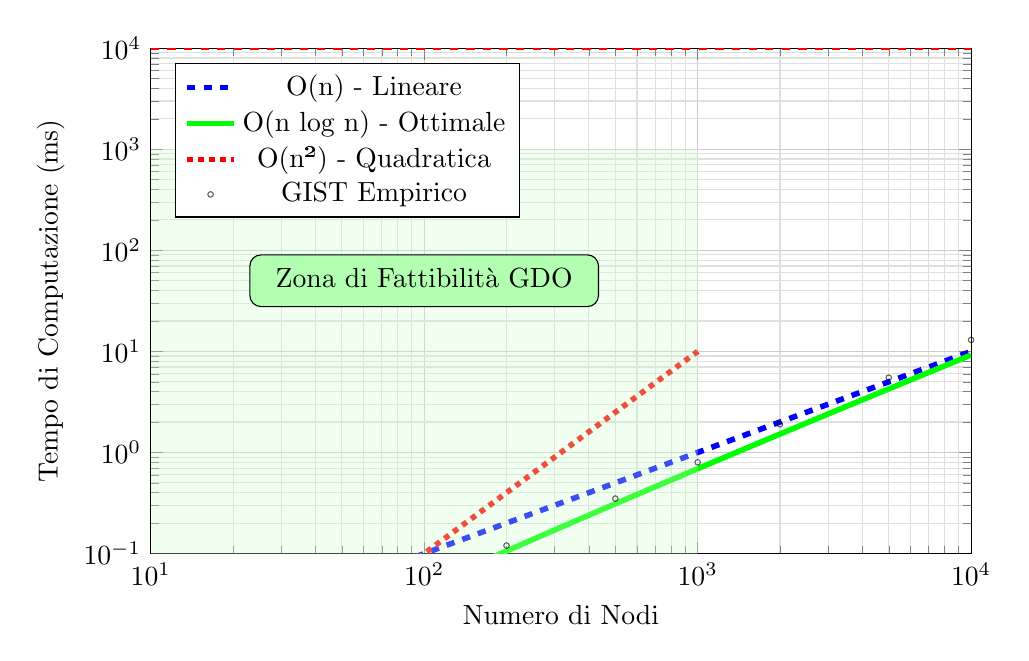
\begin{tikzpicture}
\begin{loglogaxis}[
    width=12cm,
    height=8cm,
    xlabel={Numero di Nodi},
    ylabel={Tempo di Computazione (ms)},
    xmin=10, xmax=10000,
    ymin=0.1, ymax=10000,
    grid=both,
    minor grid style={gray!25},
    major grid style={gray!40},
    legend pos=north west,
    %title={Analisi di Complessità Computazionale del Framework GIST\\{\small Confronto con Algoritmi di Riferimento}}
]

% O(n)
\addplot[blue, dashed, line width=2pt, domain=10:10000] {x*0.001};
\addlegendentry{O(n) - Lineare}

% O(n log n)
\addplot[green, line width=2pt, domain=10:10000] {x*ln(x)*0.0001};
\addlegendentry{O(n log n) - Ottimale}

% O(n²)
\addplot[red, dotted, line width=2pt, domain=10:1000] {x^2*0.00001};
\addlegendentry{O(n²) - Quadratica}

% GIST empirico (punti simulati)
\addplot[black, mark=o, mark size=1pt, only marks, opacity=0.6] coordinates {
    (10,0.003) (20,0.007) (50,0.02) (100,0.05) (200,0.12) 
    (500,0.35) (1000,0.8) (2000,1.9) (5000,5.5) (10000,13)
};
\addlegendentry{GIST Empirico}

% Area di fattibilità
\fill[green!20, opacity=0.3] (axis cs:10,0.1) rectangle (axis cs:1000,1000);
\node[draw, fill=green!30, rounded corners] at (axis cs:100,50) {
    \begin{tabular}{c}
    Zona di Fattibilità GDO
    \end{tabular}
};

% Limite pratico
\draw[red, dashed, line width=1pt] (axis cs:10,10000) -- (axis cs:10000,10000);
\node[red, above] at (axis cs:1000,10000) {\footnotesize Limite Pratico (10s)};

\end{loglogaxis}
\end{tikzpicture}
\caption{Analisi di complessità computazionale del framework GIST confrontata con algoritmi di riferimento.}
\label{fig:complessita}
\end{figure}
\end{document}